\documentclass[12pt]{article}

\usepackage{sbc-template}

\usepackage{graphicx,url}
\usepackage{amssymb}

%\usepackage[brazil]{babel}   
%\usepackage[latin1]{inputenc}  
\usepackage[utf8]{inputenc}  
% UTF-8 encoding is recommended by ShareLaTex

     
\sloppy

\title{Implementation and Analysis of Collaborative Filtering Algorithm on MovieLens Latest Small Dataset}


\author{Xinqi Zhu 5150297, Ryan Mckay z5060961}

\address{School of Computer Science and Engineering -- University of New South Wales}


\begin{document} 

\maketitle

\begin{abstract}
We present our study of recommender system's and user-item rating systems, i.e. user-movie rating system. We have focused on the most prolific algorithm in recommender systems, collaborative filtering, more specifically Latent Factor and K-Nearest-Neighbour (KNN) techniques for rating prediction and we establish a simple classification rule as a means for considering so called top N recommendations. In this report, we outline the implementation, experimentation and evaluation of our collaborative filtering solution and explore various methods to measure prediction accuracy based on experiments. 
\end{abstract}


\section{Introduction}

Recommender system's have become very popular in recent times, implemented by many Internet giants to guide customers toward products they are likely to click on, watch, purchase or consume in general. One of the most successful recommendation algorithms is collaborative filtering.

%In this project, our goal is to implement a version of collaborative filtering algorithm on a MovieLens user-movie rating dataset and do sufficient experiments to make the system work properly and give a reasonable prediction accuracy.
%
%Also we apply multiple evaluation methods to our system and see how the value of parameters change the performance of the system.

%\section{Related Work}


\section{Data Preparation}

\section{Implementation}

Our implementation includes 
\begin{itemize} 
	\item Latent factor model
	\item KNN model
	\item K-Fold cross validation
	\item Precision-Recall Curve 
	\item Performance evaluation metrics and supporting visualizations
\end{itemize}

\subsection{Collaborative Filtering Algorithm}

There are two primary areas of collaborative filtering: neighborhood methods and latent factor models\cite{MF}. Our realization of the latent factor model called matrix factorization(MF) and k-nearest-neighbor for neighborhood method.

\subsubsection{Latent Factor Model}
This algorithm will model the user-movie rating matrix as inner product of a user matrix and a movie matrix. Each movie is represented as a vector $X_i \in \mathbb{R}^f$ and each user is associated with $\theta_j \in \mathbb{R}^f$. The approximate rating by user j on movie i is:
$$\hat{r}_{ij} = X_i^T \cdot \theta_j$$

This implementation require the determination of the number of features $f$, which is used to represent the features of a movie and the preference of a user on these features. In Experimental Evaluation section we discuss the number of feature selection.

In order to get the proper $X$ and $\theta$ matrix, we use the definition of cost function from \cite{MF}:
$$J = \frac{1}{2}\sum_{(i,j):t(i,j)=1}(X_i^T \cdot \theta_j - r_{ij})^2+\frac{\lambda}{2}\sum_{i = 1}^{n_m}\sum_{k = 1}^{f}X_{ik}^{2}+\frac{\lambda}{2}\sum_{j = 1}^{n_u}\sum_{k = 1}^{f}\theta_{jk}^{2}$$
where $t(i,j)$ means movie $i$ has been rated by user $j$. $\lambda$ is the regularization coefficient and should be determined by experiment.

The gradient of $X$ and $\theta$:
$$\frac{\partial J}{\partial X_{ik}} = \sum_{j:t(i,j)=1}(X_i^T \cdot \theta_j - r_{ij})\theta_{jk}+\lambda X_{ik}$$
$$\frac{\partial J}{\partial \theta_{jk}} = \sum_{i:t(i,j)=1}(X_i^T \cdot \theta_j - r_{ij})X_{ik}+\lambda \theta_{jk}$$

Then we use the predefined optimization method of Conjugate Gradient from scipy library to train our model. In order to do so, we compress the $X$ and $\theta$ matrix into a vector to fit the minimization function.

When doing prediction, we get the inner product of $X$ and $\theta$ matrix to get $\hat{r}$ matrix. Then we replace each value in $\hat{r}$ by the nearest rating level (0.5, 1.0, 1.5 ...) and compare it with the true rating matrix $r$ (details in section 5).

\subsubsection{K-Nearest-Neighbor Model}

\subsection{K-fold Cross Validation}
We use k-fold cross validation to determine the proper number of features $f$, the regularization coefficient $\lambda$ and do any other debugging.

By using the KFold function of sklearn's model\_selection library, we can easily split the training set into k folds and use any of them as validation set. In our implementation, we take $k=5$ and use the mean of each fold's MSE(mean square error) and MAE(mean absolute error) as final training set's and CV's MSE and MAE.

\section{Experimental Evaluation}
We randomly split the raw data of user-movie rating into training set(80\%) and test set(20\%), then do experiments with k-fold cross validation with $k=5$.
The experiments include determination of the number of features $f$, regularization coefficient $\lambda$, getting learning curve and ROC(receiver operating characteristic) curve.

Figure \ref{fig:exampleFig1} and Figure \ref{fig:exampleFig1} show the  experiments to get the proper $f$ and $\lambda$ and ends up with $f=105$ and $\lambda = 1.3$. We can see when $\lambda$ is larger than 1.3 the MSE on CV set is increasing and likely to be underfitting(high bias). On the contrary, low $\lambda$ makes the system overfitting(high variance). We set $f=105$ at the elbow point because larger $f$ takes more time to train but no obvious improvement on result, and lower $f$ is not mature enough.

Figure \ref{fig:exampleFig1} shows the learning curve under three conditions: underfitting($\lambda = 5$), normal($\lambda = 1.3$), and overfitting($\lambda = 0.2$).

Figure \ref{fig:exampleFig1} shows the ROC curve of our recommender system. The confusion matrix is defined based on the assumption that the truth rating beyond a threshold should be regarded as true positive and below as true negative\cite{CF_Recsys_Survey}. For prediction, we maintain a top rating list, i.e. top 100 rating movies to be predicted positive and rest to be predicted negative. We test three thresholds, 3, 4 and 4.5 stars. We draw the curve by changing the size of the top N list.

\begin{figure}[ht]
\centering
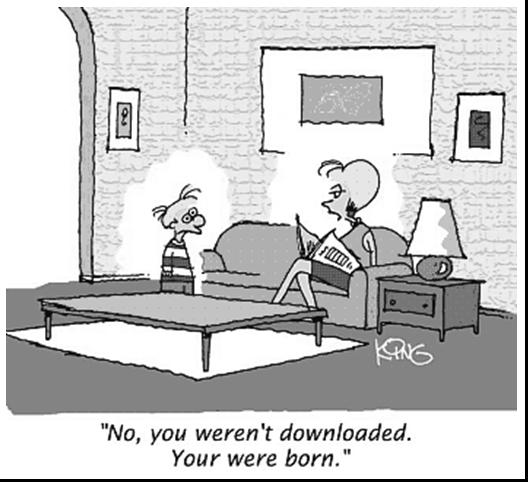
\includegraphics[width=.5\textwidth]{fig1.jpg}
\caption{A typical figure}
\label{fig:exampleFig1}
\end{figure}

\begin{figure}[ht]
\centering
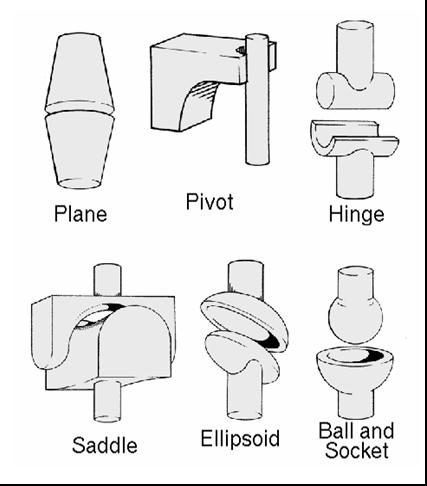
\includegraphics[width=.3\textwidth]{fig2.jpg}
\caption{This figure is an example of a figure caption taking more than one
  line and justified considering margins mentioned in Section~\ref{sec:figs}.}
\label{fig:exampleFig2}
\end{figure}

%In tables, try to avoid the use of colored or shaded backgrounds, and avoid
%thick, doubled, or unnecessary framing lines. When reporting empirical data,
%do not use more decimal digits than warranted by their precision and
%reproducibility. Table caption must be placed before the table (see Table 1)
%and the font used must also be Helvetica, 10 point, boldface, with 6 points of
%space before and after each caption.
%
%\begin{table}[ht]
%\centering
%\caption{Variables to be considered on the evaluation of interaction
%  techniques}
%\label{tab:exTable1}
%\smallskip
%\begin{tabular}{|l|c|c|}
%\hline
%& Value 1 & Value 2\\[0.5ex]
%\hline
%&&\\[-2ex]
%Case 1 & 1.0 $\pm$ 0.1 & 1.75$\times$10$^{-5}$ $\pm$ 5$\times$10$^{-7}$\\[0.5ex]
%\hline
%&&\\[-2ex]
%Case 2 & 0.003(1) & 100.0\\[0.5ex]
%\hline
%\end{tabular}
%\end{table}

\subsection{Results}

For latent factor model, our system reaches an mean square error of 0.9 and mean absolute error of 0.5. The average accuracy of correct prediction on rated movies is 70\%. This is an amazing ratio because most of the user's interaction with movies has been correctly predicted. The ROC curve shows that the prediction is much better than randomly guess.

\section{Future Work}

\section{Conclusion}

%Bibliographic references must be unambiguous and uniform.  We recommend giving
%the author names references in brackets, e.g. \cite{knuth:84},
%\cite{boulic:91}, and \cite{smith:99}.
%
%The references must be listed using 12 point font size, with 6 points of space
%before each reference. The first line of each reference should not be
%indented, while the subsequent should be indented by 0.5 cm.

\bibliographystyle{unsrt}
\bibliography{sbc-template}

\end{document}
